\documentclass[a4paper,11pt]{kth-mag}
\usepackage[T1]{fontenc}
\usepackage{textcomp}
\usepackage{lmodern}
\usepackage[latin1]{inputenc}
\usepackage[swedish,english]{babel}
\usepackage{modifications}
\usepackage[acronym, numberedsection=autolabel]{glossaries}
\usepackage[colorlinks]{hyperref}
\usepackage{graphicx}
\usepackage{nameref}

\newcommand*{\fullref}[1]{\hyperref[{#1}]{\autoref*{#1} \nameref*{#1}}} % One single link
\renewcommand*{\glsdisplayfirst}[4]{#1#4*} % Glossary first entry

\newcommand*{\captionsource}[2]{%
  \caption[{#1}]{%
    #1%
    \\\hspace{\linewidth}%
    \textbf{Source:} #2%
  }%
}

\def\mypart#1#2{% 
\par\newpage\clearpage % Page break 
\vspace*{5cm} % Vertical shift 
\refstepcounter{part}% Next part 
{\centering \textbf{\Huge Part \thepart}\par}% 
\vspace{1cm}% Vertical shift 
{\centering \textbf{\Huge #1}\par}% 
\vspace{2cm}% Vertical shift % Some text 
#2 
\vfill\pagebreak %
}
\makeglossaries

% Epigraph
%\epigraphfontsize{\small\itshape}
\renewcommand{\epigraphrule}{0pt}
\renewcommand{\epigraphflush}{flushright}
%\renewcommand{\textflush}{center}
\setlength{\epigraphwidth}{.7\textwidth}

% Glossary
\newglossaryentry{rpi}{name={runaway process inflation}, description={Runaway inflation is a very rapid inflation (decrease of money value). Runaway process inflation is a term sometimes used within agile development to describe rapidly growing development processes}}
\newglossaryentry{td}{name={technical dept}, description={Technical dept (also called design dept or code dept), is a metaphor primarily used in software development referring to the consequences of poor system design. The dept builds up as you for example introduce bugs and so called spaghetti code that has to be fixed in the future, as in repaying your dept}}
\newglossaryentry{ev}{name={Early Victory}, description={A strategy commonly referenced to in agile development that refers to the sociological benefits of showing early and frequent results, such as increasing morale and trust \cite{key6}}}
\newglossaryentry{osmosis}{name={osmosis}, description={The movement of a liquid, sometimes gas, through a plasma membrane (which is a sort of filer) which over time results in a balancing from high concentration areas to low for the molecules that are able to pass through the plasma membrane}}
\newglossaryentry{es}{name={executive sponsor}, description={Also referred to as the project sponsor. Executive sponsor is a role in project management that is responsible to the business/company for the success of a project}}
\newglossaryentry{git}{name={Git}, description={Git is a popular distributed revision control system mainly used for software development.}}
\newglossaryentry{jitg}{name={JIT}, description={Just-in-time is a production strategy that seeks to improve the return on investment for a business by reducing in-process inventory and associated carrying costs. In simpler terms, reducing the stock up of inventory items in a process chain.}}
\newglossaryentry{roig}{name={ROI}, description={Return on investment means the benefits, or return, for the investor resiling from an investment of some resource. High ROI}}




% Acronyms
\newglossaryentry{jit}{type=\acronymtype, name={JIT}, description={just-in-time}, first={just-in-time (JIT)\glsadd{jitg}}, see=[Glossary:]{jitg}}
\newglossaryentry{roi}{type=\acronymtype, name={ROI}, description={return-on-investment}, first={jreturn-on-investment (ROI)\glsadd{roig}}, see=[Glossary:]{roig}}
\newacronym{tdd}{TTD}{test-driven development}
\newacronym{gui}{GUI}{graphical user interface}
\newacronym{wip}{WIP}{work-in-progress}
\newacronym{xp}{XP}{Extreme Programming}
\newacronym{lsd}{LSD}{lean software development}
\newacronym{lpd}{LPD}{lean product development}




\title{Agile Development in a Solo Environment}

\subtitle{Duis autem vel eum iruire dolor in hendrerit in
          vulputate velit esse molestie consequat, vel illum
          dolore eu feugiat null}
\foreigntitle{Lorem ipsum dolor sit amet, sed diam nonummy nibh eui
              mod tincidunt ut laoreet dol}
\author{Mathias Lindblom}
\date{June 2015}
\blurb{Master's Thesis at KTH Royal Institute of Technology\\Computer Science and Communication (CSC)\\Supervisor: Sten Andersson\\Examiner: Olle B�lter}
 \trita{}
\begin{document}
\frontmatter
\pagestyle{empty}
\removepagenumbers
\maketitle
\selectlanguage{english}
\begin{abstract}
  This is a skeleton for KTH theses. More documentation
  regarding the KTH thesis class file can be found in
  the package documentation.

Lorem ipsum dolor sit amet, consectetuer adipiscing elit. Mauris
purus. Fusce tempor. Nulla facilisi. Sed at turpis. Phasellus eu
ipsum. Nam porttitor laoreet nulla. Phasellus massa massa, auctor
rutrum, vehicula ut, porttitor a, massa. Pellentesque fringilla. Duis
nibh risus, venenatis ac, tempor sed, vestibulum at, tellus. Class
aptent taciti sociosqu ad litora torquent per conubia nostra, per
inceptos hymenaeos.
\end{abstract}
\clearpage
\begin{foreignabstract}{swedish}
  Denna fil ger ett avhandlingsskelett.
  Mer information om \LaTeX-mallen finns i
  dokumentationen till paketet.

Lorem ipsum dolor sit amet, consectetuer adipiscing elit. Mauris
purus. Fusce tempor. Nulla facilisi. Sed at turpis. Phasellus eu
ipsum. Nam porttitor laoreet nulla. Phasellus massa massa, auctor
rutrum, vehicula ut, porttitor a, massa. Pellentesque fringilla. Duis
nibh risus, venenatis ac, tempor sed, vestibulum at, tellus. Class
aptent taciti sociosqu ad litora torquent per conubia nostra, per
inceptos hymenaeos.
\end{foreignabstract}
\clearpage
\tableofcontents*
\mainmatter
\pagestyle{newchap}

\chapter{Introduction}
This chapter will initially go through the problem statement and goals of the report. It will also show the motivation and estimated value of the entire report. The last section will outline the structure of the rest of the report.

Agile development is something

\section{Problem Statement}
Agile software development can be seen as a trend in today's computer industry and the actual concept of the method changes every year, which is quite appropriate given what the methodology advocates. The method mainly targets advanced systems and encourage continuous improvement and rapid changes to new customer demands. The development process revolves around having collaboration between self-organizing and cross-functional teams with focus on communication together with a iterative development process. However the information available regarding how-to practically establish an agile development process in small companies with small projects is limited. The available literature usually give hints on where to start but focuses heavily on the full blown methodologies and leaves it up to the reader to decide what is practically possible for their limited sized development group or company.

This can make it hard and confusing for developers wanting to adopt an agile mindset when starting their new company with only a few people or even by themselves. Moreover, trying to follow most agile methodologies, or other methodology types for that matter, completely can be overwhelming and lead to unnecessary abandonment of that methodology. By finding a good approach to how small teams and/or companies can adopt agile software development, future problems such as communications issues or delays that comes from not following a methodology can be avoided.

\section{Motivation \& Value} %syfte

\section{Goals}
The main goal of the thesis is as follows:

\begin{itemize}
\item Find agile development methodologies or agile strategies suitable for a single developer up to small teams consisting of only a handful of people.
\end{itemize}
\noindent
Secondary goals:

\begin{itemize}
\item Theoretical comparison of popular agile development methodologies.
\item Overall clarification of agile terms and thinking/reasoning. For example differentiate Agile from Lean.
\item Produce a working prototype of the interactive tutoring framework described later. This is also the main goal of the project owner, Per-Arne Forsberg.
\end{itemize}

\section{Limitations}

\section{Thesis Report Outline}

\mypart{Background} {The following two chapters forms the base for the theoretical and practical part of this reports study. The first chapter explains agile development as a concept and its core ideas. The second chapter explains some of the most common agile methodologies, by mainly going through their practices.}

\chapter{Agile Development}
\label{sec:agile_development}

Most developers have experienced the nightmare of working on a project and slowly witness the increasing number of bugs, errors and time when adding new functionality. In order to combat this disheartening scenario, developers tend to create constraints and routines around their activity, forming a development process based on prior mistakes. However big development projects can be complex and even though experienced based constraints helps, the problems remains and builds upon each other. One solution for this is to keep adding more constraints and routines. So the development process grows and grows and until the process itself becomes so cumbersome and advanced that it creates the problems it was designed to prevent, which was to avoid \gls{td} and increase efficiency \cite{key1}. 

This so called \gls{rpi} was common among big companies around the millennium shift and at the time it was a growing negative trend \cite{key1}. Software teams around the world experienced this, including a few industry experts calling themselves the Agile Alliance who sought to fight it \cite{key1}. The ideas that make up agile development were not new at the time but it was the Agile Alliance that formulated the underlying concepts that make up agile development. The report will come back to this at \fullref{sec:manifesto}.

\section{Component Abstraction}
\label{sec:abstraction_components}
It is common that agile development is directly compared to the waterfall model which is strange given how they situate on different abstraction levels. What this means is that the waterfall model is a software development methodology just like Scrum. Agile development on the other hand is not a followable methodology by itself. It is more of an ideology or perhaps a collection of methodologies. So how is it even possible to compare the two of them? The answer is that people are comparing the waterfall model to some popular agile methodology like Scrum or some common practices like sprints and standup meetings, indirectly claiming that these elements represent agile development as a whole. This leads to confusion and unfair comparisons. So before continuing reading about agile development it is a good idea to give a short overview of the components that make up agile development. Bare in mind that this is a simplified overview meant to give the reader a better sense of how agile development and the methodologies with its practices correlate to each other.

In Figure \ref{fig:agile_abstraction}, agile development have been dividid into four different abstraction levels. First we have the ideology that consist of the core ideas such as The Agile Manifesto and principles. This is basically what defines agile development. Secondly we have the methodologies and strategies that fulfills some or all of the agile principles and philosophies. The third abstraction are the practices that make up the methodologies, similar to how the principles make up agile development. However, the practices are more practically applicable and at a much lower abstraction level. Lastly, at the forth abstraction level, we have the actual tools that are needed to make the practices a reality. These tools can be very simple such as a physical room for meeting practices or more advanced such as the xUnit framework for test-driven development.

The report will frequently talk about these different components so it is a good idea to keep a mental image of Figure \ref{fig:agile_abstraction}. Moreover, this report will refer to agile development as an ideology in order to not confuse it with the methodologies.

\begin{figure}[h]
  \centering
    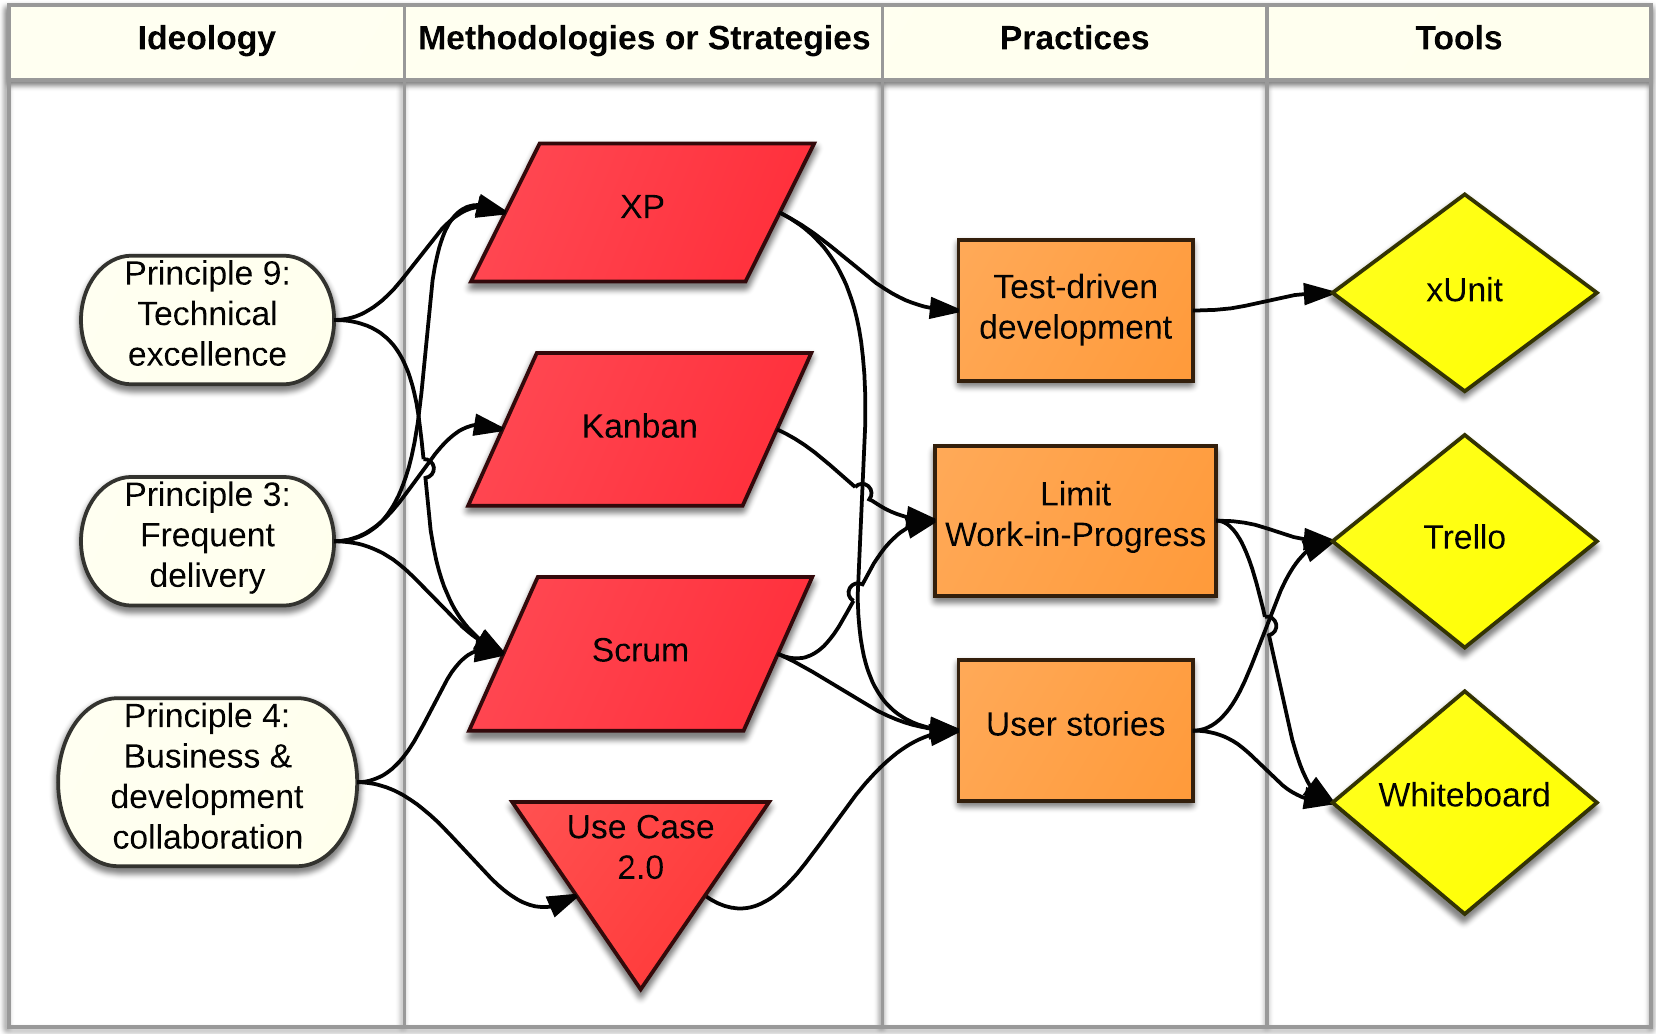
\includegraphics[width=1.0\textwidth]{img/agile_development_abstraction.png}
    \caption{Agile development divided into four different abstraction levels starting with the ideology that defines agile development and ending with physical tools. It also shows how the example elements within them correlate to each other.}
    \label{fig:agile_abstraction}
\end{figure}

\section{The Agile Manifesto}
\label{sec:manifesto}
The Agile Alliance is an organization formed by a group of computer industry experts in 2001. They decided to come together to form general development values in order to improve the software development process for companies around the world and to give an alternative to the popular heavyweight methodologies \cite{key1} \cite{key2}. The result was The Agile Manifesto that states the following:

\begin{itemize}
\item \textbf{Individuals and interactions} over processes and tools.
\item \textbf{Working software} over comprehensive documentation.
\item \textbf{Customer collaboration} over contract negotiation.
\item \textbf{Responding to change} over following a plan.
\end{itemize}

The group that wrote The Agile Manifesto consisted of the following people: Kent Beck, Mike Beedle, Arie van Bennekum, Alistair Cockburn, Ward Cunningham, Martin Fowler, James Grenning, Jim Highsmith, Andrew Hunt, Ron Jeffries, Jon Kern, Brian Marick, Robert C. Martin, Steve Mellor, Ken Schwaber, Jeff Sutherland, Dave Thomas \cite{key1} \cite{key2}. Several of these people are the authors of the literature used in this report, this is especially true for \fullref{sec:agile_methodologies}.

The following four subsections will give a short explanation for each of the statements of The Agile Manifesto that stands as the highest abstraction or the core that is agile development.

\subsection{Individuals and Interactions over Processes and Tools}

\epigraph{Process and technology are a second-order effect on the outcome of a project. The first-order effect is the people. \cite{key1}}{\textsc{Alistair Cockburn}}
\noindent
Within football most agree that a football team of average players that communicate well can beat a team of egoistic superstars. The same goes for software development (and probably many more things) where a team of average programmers working together outperforms a team of expert programmers that fail to communicate. At least according to the thinking and reasoning of agile development \cite{key1}.

Processes and tools are of course important as well but not as important. After all, agile development methodologies are processes that usually requires tools. Team managers have a habit of setting up the development environment and then assigning a team, assuming that the team will work well since they have the tools they need \cite{key1}. However this is focus put at the wrong end of order. Tools and processes can rarely repair a team that doesn't play ball but a functioning team is usually capable of configuring their own environment \cite{key1}.

\subsection{Working Software over Comprehensive Documentation}

\epigraph{The program is the specification and documentation. \cite{key3}}{\textsc{Douglas Crockford}}

\noindent
This might not be that much of a shocker, that functioning software is more important than documentation. The keyword here is \emph{comprehensive} since it is common that teams get hung up on the quest of having close to 100 percent coverage on documentation \cite{key1}. The problem with this is that it takes a lot of time and effort to always keep in sync with the code and as soon as you lose the sync, the documentation begins telling lies. Instead of having every technical part of a program described in a thick book it is usually preferred, both for the reader and the writer, to have a short rational and structured document that explains the software at a high abstraction. When a new member of a team needs more technical information they will get it when working closely and interacting with their team members and the actual software \cite{key1}.

A common misconception is that code is for the computer and documentation for the human to understand the code \cite{key4}. Instead of translating the code into human language, why can't we write code so that humans can understand it in the first place? We already do it by naming things like classes and methods with understandable names, but is usually ends there. We make it \emph{good enough}. If we instead focused more on the quality and logic of the code, a comprehensive documentation should not be needed at all. 

\subsection{Customer Collaboration over Contract Negotiation}
Many have tried to create strict contracts with fixed specifications, deadlines and prices for software development. Many have failed \cite{key3}. You simply can't treat software as a commodity expecting everything to be known before hand. Trying to do so can lead to all sorts of avoidable problems like poor quality or even complete failure. It is not only the complexity of programming that is the issue but also how fast our technical world changes over short time periods. This is one of the core problems that agile development tries to avoid. By having a tight collaboration with the customer, the specifications, deadlines and prices don't need to be as strict. Instead of having a contract specifying the exact requirements of the entire project it should instead address how the collaboration between customer and developers should be conducted \cite{key3}. This leads to a more dynamic development approach where technical problems can be addressed directly. More over, needed changes don't risk breaking the contract.

\subsection{Responding to Change over Following a Plan}	
Some of the reasons for this priority is stated in the previous  section regarding customer collaboration. Customers have a habit of not knowing what they really want or change their requirements after seeing some of the functionality coming to life \cite{key3}. Also like stated in the previous section about collaboration, the IT world we live in rapidly changes and so can the requirements of a software project. It is nice and tempting to have the full project planned in some advanced planning software with every functionality written. However as the development team and customer moves forward the plan is bound to change. Some functionality will no longer be deemed necessary and previously unthought of functionality might be added. Some parts of the strict plan might then have been a waste of time and more importantly, the strict plan might hinder these kind of positive changes that are needed or are advantageous to the project. 

By having a more abstract and lose plan with details only for the near future, for example a couple of weeks, you get a planning more susceptible to change \cite{key3}. That detailed plan can be strict but since it is only for a short time period the risks of having unneeded functionality or hindering change is limited. The further away in time we look the weaker the plan should be since we want flexibility to changes and the likelihood of changing requirements grows as the timeline increases.

\section{The Agile Principles}
\label{sec:agile_principles}
Using the values stated by The Agile Manifesto, 12 principles were created that act as the characteristics for agile practices \cite{key1}. You can interpret these principles as the next abstraction step from The Agile Manifesto where you get a clearer explanation of what agile development is. These are the principles:

\begin{enumerate}
\item Our highest priority is to satisfy the customer through early and continuous delivery of valuable software.
\item Welcome changing requirements, even late in development. Agile processes harness change for the customer's competitive advantage.
\item Deliver working software frequently, from a couple of weeks to a couple of months, with a preference to the shorter timescale.
\item Business people and developers must work together daily throughout the project.
\item Build projects around motivated individuals. Give them the environment and support they need, and trust them to get the job done.
\item The most efficient and effective method of conveying information to and within a development team is face-to-face conversation.
\item Working software is the primary measure of progress.
\item Agile processes promote sustainable development. The sponsors, developers, and users should be able to maintain a constant pace indefinitely.
\item Continuous attention to technical excellence and good design enhances agility.
\item Simplicity--the art of maximizing the amount of work not done--is essential.
\item The best architectures, requirements, and designs emerge from self-organizing teams.
\item At regular intervals, the team reflects on how to become more effective, then tunes and adjusts its behavior accordingly.
\end{enumerate}


%\section{Misconceptions}
%Skeptics to agile development sometimes claim that agile development is just a trend, a so called fad. However the %arguments are similar to the time when people claimed the world wide web to be a youthful trend. It is a sort of straw man %argument based on that it is new and popular and will soon disappear, just like trends. 
%It is sort of a dictatorship vs democracy, dictatorship works but not well enough. And for a democracy to work the people %need to be onboard. 

\section{Agile vs Waterfall}
This section will a short illustrative and abstract view of the difference between agile development and the more established software development methodology called the waterfall model. As explained in \fullref{sec:abstraction_components}, one should be careful doing detailed comparisons between agile development and other methodologies since agile development is a bundle of methodologies.

As seen in Figure \ref{fig:agile_waterfall}, the waterfall model takes one logical project step and finishes it before starting the next step, like sequential waterfalls that moves the project from one logical plane to the next. Each team work on different projects at any given time and each team work on one part of the project chain. Which means that the implementation team does not care about design for example. In Figure \ref{fig:agile_waterfall}, when the design team is finished with project 2 it gives the project to the implementation team and waits for a new project to arrive from the planning team. 

In agile development, the project does not normally move from one distinct team to another. Instead, one team holds a project until it is completely finished before starting work on another project. For a team to be able to hold a project from start to finish it is vital that entire team incorporates all necessary skills within a project, which normally is done through so called cross-functional teams that are often mentioned within agile development. If another project starts, another cross-functional team is assigned that project. 

 \begin{figure}[h]
  \centering
    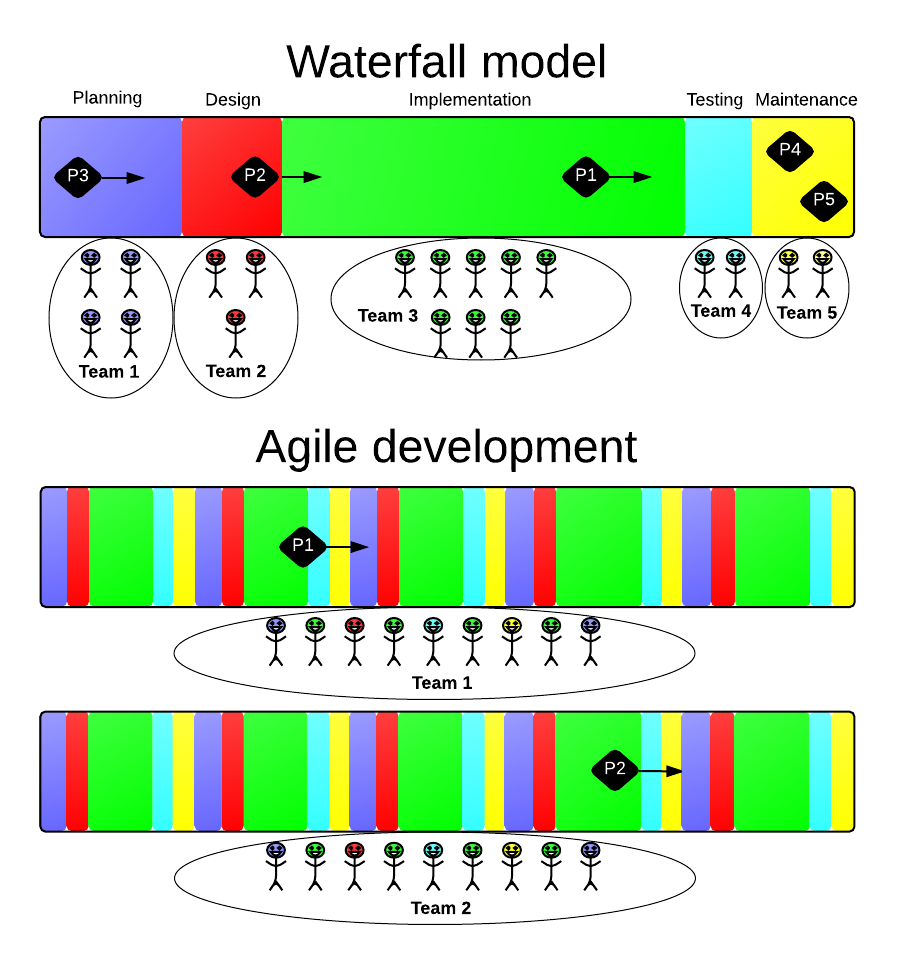
\includegraphics[width=1.0\textwidth]{img/agile_waterfall.png}
    \caption{Simplified abstract image showing the difference between the waterfall model and agile development. The image portrays how projects move forward in an arbitrary timeline through difference phases. P1 to P5 stands for Project 1 to Project 5.}
    \label{fig:agile_waterfall}
 \end{figure}

\section{Agile vs Lean}
When you read about different software development methodologies they can sometimes be referred to as \emph{lean}, sometimes \emph{agile} and sometimes times \emph{lean and agile}. Often without explanation of what specific parts makes the methodology lean and what makes it agile which can be very confusing. To understand the confusion it is best to give a short explanation of what lean development means:
\begin{description}
\item[Lean] \hfill \\
\gls{lpd}, or Lean manufacturing, dates back to the mid 20th century. The history of \gls{lpd} begins with Toyota that sought to improve manufacturing efficiency, quality and flexibility. One way to achieve this, according to \gls{lpd}, is to have the entire chain from design to full assembly at one physical place \cite{key22}. This is comparable to how agile development promotes having short iterations where all parts of the software development chain is incorporated. 

\gls{lsd} is simply the adaptation of \gls{lpd} to the software industry that originates from the book  \emph{Lean Software Development: An Agile Toolkit} by Mary Poppendieck and Tom Poppendieck \cite{key23}. Like with agile development, \gls{lsd} has a few principles that gives a good overview of what the methodology or ideology is about:

\begin{enumerate}
\item Eliminate waste
\item Amplify learning
\item Decide as late as possible
\item Deliver as fast as possible
\item Empower the team
\item Build integrity in
\item See the whole
\end{enumerate}
\end{description}
 
Note that \gls{lsd} has just over half the amount of principles compared to agile development. Without going into detail for each specific principle we can see that several of the lean principles have similarities to the agile principles. L1 says to remove waste while A1 says to maximize value. L2 is hidden in several of the agile principles. L3 is about delaying decisions as late as possible to make the best informed decision which is a simplified version of A2. L4 and A3 both talks about fast delivery. L5 is basically what A5 states.

So by looking at the principles it is safe to say that the lean and agile ideologies have several similarities. They both talk about adaptive planning, empowering the people, fast delivery, continuous improvement etcetera. The differences lies in focus and scope that becomes more apparent when reading literature about them. \gls{lsd} focuses on minimizing waste and streamlining workflow while agile development focuses on adaptivity and communication. \gls{lsd} reaches a higher range than agile software development by going all the way to talk about costumer vision, staffing and maintenance while agile development has a more strict focus on the project development phase. 

What is important to note is that agile and lean do not go against each other. This means that methodologies trying to adopt these ideas do not have to be either agile or lean but can in fact be both, with perhaps a focus towards one of them. This chapter will end with a suitable long quote from one of the authors of the agile manifesto.

\epigraph{So as you can see, lean and agile are deeply intertwined in the software world. You can't really talk about them being alternatives, if you are doing agile you are doing lean and vice-versa. Agile was always meant as a very broad concept, a core set of values and principles that was shared by processes that look superficially different. You don't do agile or lean you do agile and lean. The only question is how explicitly you use ideas that draw directly from lean manufacturing.}{\textsc{Martin Fowler} \cite{key24}} 


\chapter{Agile Methodologies}
\label{sec:agile_methodologies}
Up to this point the ideology, that is agile development, have been described. In this chapter the more common methodologies that try to adapt these ideas and mentalities will be brought up. Moreover, the methodologies described here will contain more practically applicable agile practices. What is important to note is that every agile methodology is subject to change. Most authors and advocates of the agile methodologies encourages changes in the methodology itself to suit your development team and/or company. This means that the descriptions of the methodologies can look more or less different depending on the source, especially when they have been written years apart. Another reason is that some parts of a methodology can be vague resulting in different interpretations. However this does not necessarily mean that some descriptions of the practices are wrong. The vagueness can be seen as a way of encouraging changes and alternative implementations of the methodologies which the authors advocates.

The methodologies can be vast in their documentation and this report does not seek to explain each methodology in their deepest details. That would simply require to much work and be overwhelming for the readers. For the interested reader, each methodology will have recommended further reading in its introduction. One thing that every agile methodology has in common is a set of practices that explain the most important components. Some methodologies refer to them as properties but they all seek to explain the core of the methodology similar to how the agile principles, in \fullref{sec:agile_principles},  relate to agile development. It was therefor suitable to use them as the base for this reports overview of the methodologies in order to ensure that the description and comparisons are based on somewhat equal grounds. Each methodology section will end with short summarize of the practices.

A warning to the readers is that going through every practice of all four methodologies in order might be quite heavy reading. An alternative suggestion is to read the practice titles and go back to read the content when needed as the report starts investigating the practices at \fullref{sec:method_teori}.

\section{Scrum}
Scrum is one of the most known and used agile methodologies today. Scrum was originally codeveloped during the early 1990s by two of the soon-to-be authors of The Agile Manifesto, Jeff Sutherland and Ken Scwaber \cite{key21}. Several other mentionable people, such as Mike Beedle, have further contributed to the development of Scrum. Since the agile methodology Scrum was conceived before The Agile Manifesto and by several of the authors, it is perhaps not that shocking that people sometimes wrongfully put an equality mark between agile development and Scrum.

Scrum is sometimes described as a framework. This is a suitable term since it has a clear structure on most aspects of a software development process, see Figure \ref{fig:scrum}, but don't describe the details for each individual part in the process chain. Scrum has distinct roles, which are part of the practices described, with heavy interaction and communication in between them. Scrum goes against the traditional predictive way of developing and instead has a more empirical approach. What this means is that Scrum assumes that problems and challenges can't be foreseen in software development. Therefor focus lies maximizing the development teams ability to deliver quickly and respond to changing requirements.

The information regarding the practices of Scrum is mainly taken from the book \emph{Agile Project Management with Scrum} by Ken Schwaber, one of the authors of The Agile Manifesto, together with updated information from \url{www.scrumguides.org} \cite{key21} \cite{key15}.

 \begin{figure}[h]
  
  \centering
    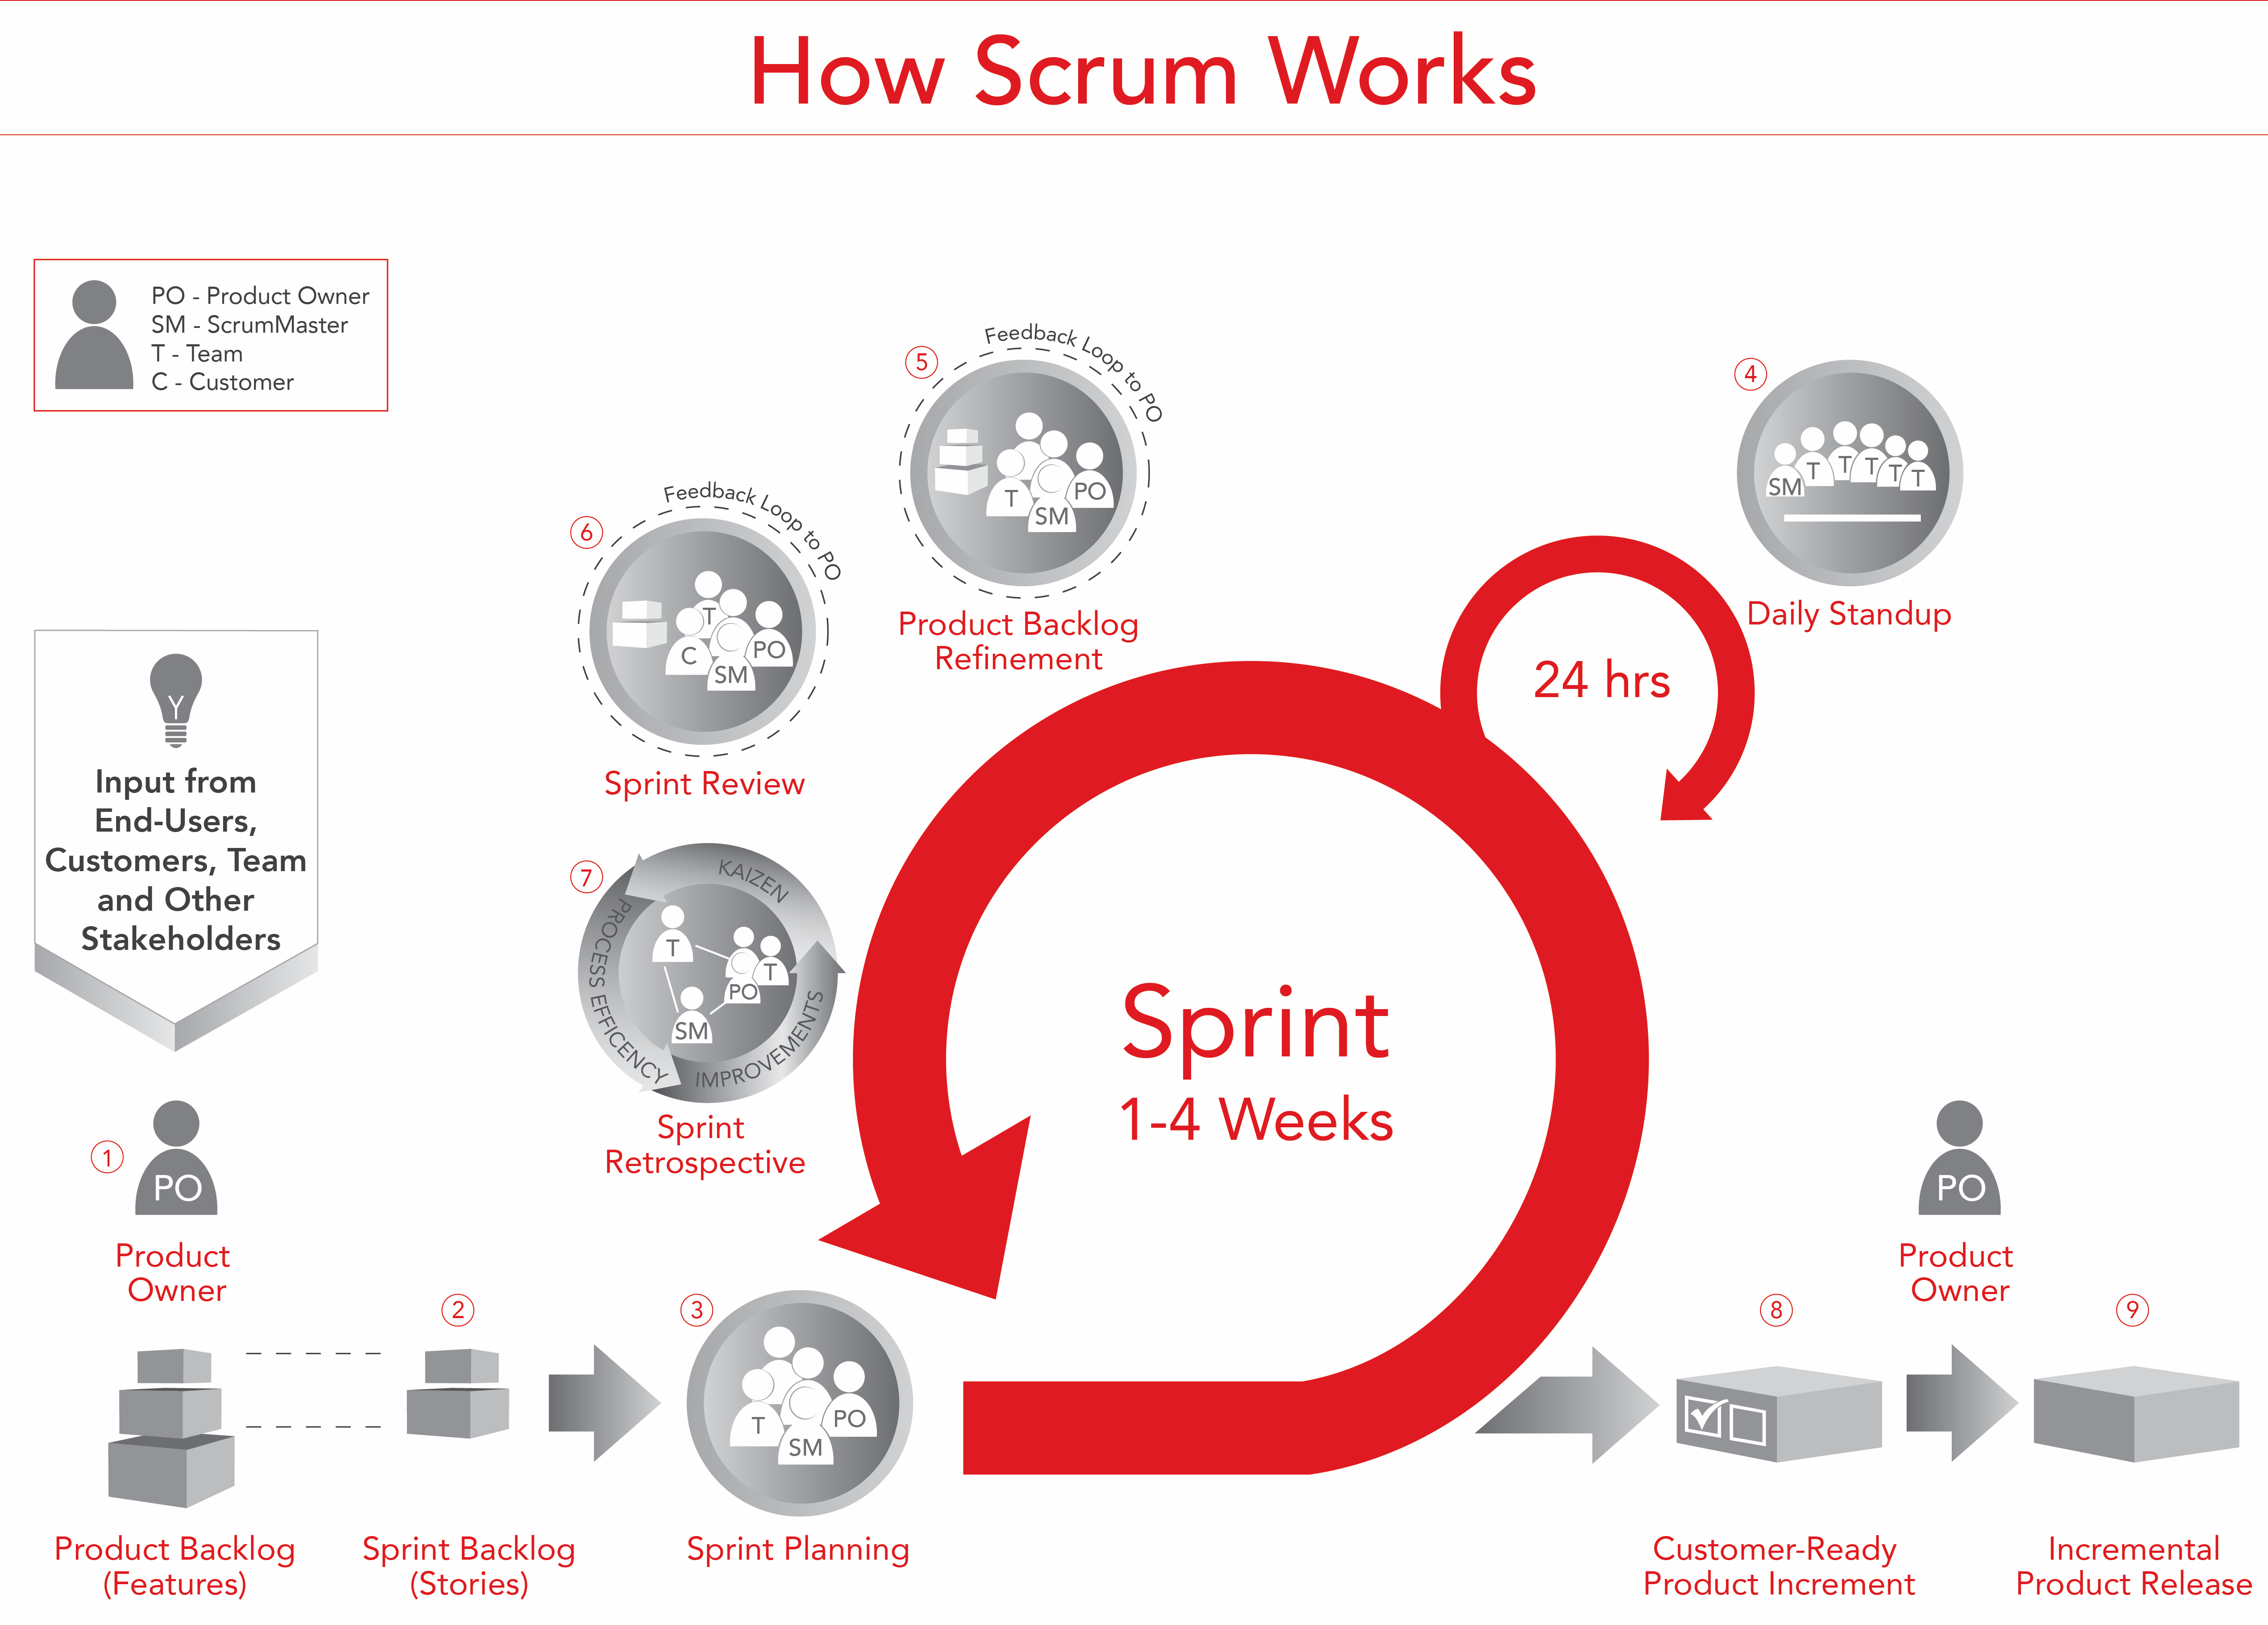
\includegraphics[width=1.0\textwidth]{img/how_scrum_works.png}
    \captionsource{Image showing an abstract view of how Scrum works, including different several practices including the three different roles.}{Scruminc, \url{http://www.scruminc.com}}
    \label{fig:scrum}
 \end{figure}

\subsection{Roles}
There are three distinct roles in Scrum. The \emph{Product Owner}, \emph{Development Team} and \emph{Scrum Master}. It is the cooperation and relation between these roles that make up Scrum. The scrum team consists of every member within these three roles.

\subsubsection{Product Owner}
The product owner is a single person. He/she is responsible of maximizing the work conducted by the \emph{Development Team} which in turn means responsibility to maximize the product value. The practical priority is managing the�\emph{Product Backlog}. The managing of the backlog means taking care of the following;

\begin{itemize}
\item Ensuring that the \emph{Product Backlog} items have clear and distinct descriptions.
\item The ordering of backlog items to maximize value and reaching goals.
\item Optimization the value of the work by the \emph{Development Team}.
\item Making the \emph{Product Backlog} visible, transparent, clear to all project members and include information about the upcoming tasks.
\item Having the \emph{Development Team} on a satisfactory level of understanding of the items in the \emph{Product Backlog}
\end{itemize}

Depending on the size of the project and company. The product owner may choose to distribute some of tasks to other people such as the development team. However, the product owner is always the accountable person for the above tasks \cite{key15}.

\subsubsection{Development Team}
In Scrum the development team are in charge of delivering working software, as one might expect. They are in a large sense self governed and chooses how they want to work, within some limits of course. 
The development team can be summarized with these characteristics:

\begin{itemize}
\item Self-organizing. The development team alone chooses how they want to turn the items in the \emph{Product Backlog} into functionality.  
\item Cross-functional. The team should encompass all necessary skills to work with everything in the \emph{Product Backlog}.
\item No titles within the group. Everyone is simply a developer.
\item No sub-teams. Just like there are no titles for the members, there can be no sub-teams such as a testing team.
\item All for one, one for all. Members might have specialized knowledge giving them natural areas of focus but the development team should be accountable as a whole.
\end{itemize}

It is recommended that each development team consist of 3-9 members \cite{key15}. The reason being that too few developers limits the interaction and the team are more likely to have skill constraints. To many members lead to too much complexity that can make coordination between the members difficult. 

\subsubsection{Scrum Master}
Deciding as a company to use a methodology and once explaining how the methodology works to all employees does not mean that the company will be developing according to that methodology. This is where the Scrum master comes in. The Scrum master is in charge of keeping the Scrum wheel turning. He/she makes sure that the \emph{Product Owner} and \emph{Development Team} are collaborating and generally doing what they are supposed to do. The following is a short summarization of the responsibilities of the Scrum master:

\begin{itemize}
\item Remove barriers regarding development so that the \emph{Product Owner} is free to directly drive development forward.
\item Teach the \emph{Product Owner} how to maximize \gls{roi} in order to meet his/her milestones using Scrum. 
\item Improve the quality of life for the \emph{Development Team} by empowering them and encouraging creativity.
\item Assist the \emph{Development Team} in increasing productivity in any way possible.
\item Ensure that each increment of functionality is potentially shippable by improving engineering practices and tools.
\item Give transparency to the \emph{Development Team's} work progress for all parties and ensure it is up-to-date. 
\end{itemize}

The position of the Scrum master is normally filled by the project manager \cite{key21}. Ken Schwaber indicates in his book,\emph{Agile Project Management with Scrum}, that a Scrum master should be a leader figure and never act as a regular boss \cite{key21}. 

\subsection{Events}
In scrum there are five so called events. However the first event called Sprint is the most important one and all the other events are basically a part of the Sprint.

\subsubsection{Sprint}
As seen in Figure \ref{fig:scrum} the sprint is very central in Scrum. The sprint is a short period of time, usually a couple of weeks up to a month \cite{key21}. As soon as one sprint ends, another starts. The sprint is about dividing the entire project into small iterations. The length of a sprint should be small enough to avoid complexity but large enough to avoid to much project overhead. The following four practices are all parts of the sprint and describes more in detail what the sprint is about, which can all be seen in Figure \ref{fig:scrum}.

\subsubsection{Sprint Planning}
Each newly starting sprint is initialized with a sprint planning. The entire scrum team should be present during this planning. The \emph{Product Owner} brings up the \emph{Product Backlog} and its priorities. These are discussed by all parts and the \emph{Development Team} goes through what will be achievable for the next sprint. So to summarize the planning is about deciding what should be done and what can be done for the coming sprint. The meeting usually has a time limit of 8 hours \cite{key21}.
\subsubsection{Daily Scrum}
Also referred to as daily standup as seen in \ref{fig:scrum}. This is something that the \emph{Development Team} does every day and should take around 15 minutes \cite{key21}. They do this to synchronize and coordinate their work efforts. There are three important questions to be answered during this meeting which are: What work have each member done since the last daily scrum? What is everyone planning on doing before the next daily scrum? What hinders exist that stand in the way of the team meeting the current sprint goals? It is the \emph{Scrum Master's} job to enforce that the daily scrum takes place and that it is only the members of the \emph{Development Team} that participate \cite{key15} \cite{key21}.
\subsubsection{Sprint Review}
The spring review is held close to the end of a sprint. The entire scrum team should be present and if possible the stakeholders as well. This is supposed to be an informal meeting where the added functionality from the sprint is shown. The \emph{Development Team} shows what they have done and the \emph{Product Owner} shows what has happened to the \emph{Backlog}. The idea is to have a revised \emph{Product Backlog} at the end that can be used for the next Sprint \emph{key15}. The durations of this meeting is usually limited to four hours \cite{key21}.
\subsubsection{Sprint Retrospective}
The spring retrospective should take place before the \emph{Sprint Planning} but after the spring review. Once again the entire scrum team is present, but without the stakeholders. This meeting should take about three hours \emph{key21}. The focus of this meeting is to improve the work process during a sprint. The team reflects about things like tools, relationships, processes and anything else that can improve the workflow of the team and sprint.

\subsection{Artifacts}
The three artifacts are the most basic parts in Scrum that are worked on during the different events.

\subsubsection{Product Backlog}
The Product Backlog is the dynamic requirements list in Scrum. It is a item list comprising of anything that can add any form of value to the product. Typical items in a Product Backlog are new features, bugs, enhancements and functions. Each Product Backlog item also has certain attributes such as a description, priority order, complexity estimate and value estimate. 

What separates a Product Backlog from a simple requirements list is that it is a dynamic process and not a static list. The items in the Product Backlog that are to be considered for the "near future", as in having a high priority order, usually have more details than other items. This is to allow changes to the distant Product Backlog items as the actual product developes.  The Product Backlog is in focus for both the practices Sprint Planning and Sprint Review. The refinement of the Product Backlog items is sometimes counted as a practice by itself as seen in Figure \ref{fig:scrum}, however the items can be tuned and refined at any time. All members of the Scrum team have a saying when it comes to the Product Backlog but the Product Owner is the main responsible person.

\subsubsection{Sprint Backlog}
The Sprint Backlog is the selected items from the Product Backlog for the ongoing Sprint. It is the list of work to be done during the Sprint. All items in this backlog have clear details since the idea is to have them all completed at the end of the Sprint, which is a relatively short time period. The Sprint Backlog changes during a Sprint as the items become implemented and moved to "done". New items can also be added as unforeseen needed functionality is added. It is the Development Team that work with the Sprint Backlog and uses it as their progress report and todo list for the current Sprint. At each Daily Scrum the Sprint Backlog is updated and refined with informations such as remaining work hours. 

\subsubsection{Product Increment}
A Product Increment is the sum of all implemented Sprint Backlog items for a Sprint. It is a sort of next "step" for the product. The requirements for a a item to counted in the Product Increment is that it is fully usable for the product. Regardless if the Product Owner chooses to release it or not, it is still counted in the Product Increment.


\section{Extreme Programming (XP)}
\glsreset{xp}
Kent Beck is the founder of \gls{xp}. He is also one of the members of the Agile Alliance that you can read about at \fullref{sec:manifesto}. \gls{xp} was conceived shortly before the creation of the Agile Alliance. In 2000, just a year before the Agile Alliance surfaced, the first book about \gls{xp} called \emph{Extreme Programming Explained: Embrace Change} was published by Kent \cite{key14}. For this reason, when reading early literature about \gls{xp} their is no mentioning of the term \emph{agile}, which is  not that strange since at the time, the term did not exist. However more published articles and books have surfaced after the year of 2001 that have incorporated the agile ideology, such as the second edition of Kent's first book realized in 2005 \cite{key14}.

Unlike Scrum, \gls{xp} is mostly about the developers and helping them be as efficient as possible. It does not talk much about the overall business outside the development team. All though if you read further about \gls{xp} you will find business related information but it is not at all in focus \cite{key14}.�\gls{xp} is usually referred to a lightweight methodology however the word \emph{lightweight} means more than just skipping business related topics. It is also called lightweight because it promotes removing baggage for the developers by letting them focus on the current task at hand \cite{key14}. For example, a core idea in \gls{xp} is small fact based short term planning instead of extensive speculation based long term planning \cite{key14}. This just happens to be one of the absolute core ideas in agile development as well. 

\gls{xp} put focus on team work, feedback and code quality. The term extreme comes from the idea that it takes a few ordinary development practices and impose them to an extreme \cite{key14}. Originally \gls{xp} was designed for small to medium sized teams but has over time grown to incorporate large teams as well. There are a total of 12 main practices in \gls{xp} that will be shortly described in the following sections. The practices have been divided in categories called \emph{Fine-Scale Feedback}, \emph{Continues Process}, \emph{Shared Understanding} and \emph{Programmer Welfare}. There are several corollary practices as well that talk more about the business and goes even further into coding details. To read about this and much more, the second edition of \emph{Extreme Programming Explained: Embrace Change} is recommended \cite{key14}.

\subsection{Fine-Scale Feedback}
The following practices describes how the members of the team develop their software with feedback in focus. It goes through the basics of how they work in pairs and always using \gls{tdd} to guide them. It also describes the relations between business people and developers.

\subsubsection{Pair Programming}
This is perhaps the most notable feature or practice regarding \gls{xp}. \emph{Pair Programming} means that for each developer, there is a another developer observing and assisting without coding. They work together similar as in rally racing where one person is the driver and one is the map reader. The main difference is that in \emph{Pair Programming} the coders switch places regularly. The purpose is that the observing developer can have their mind set on a higher abstraction level and is not distracted by coding, making it easier to ensure high code quality \cite{key1}. Not only are bugs detected more easily but the overall resulting code is simply put better. This way of developing can be quite motivating for the developers since you are never alone and if you grow tired of typing you just switch places with your pair. If the developers also switch partners every other day, information and knowledge is spread rapidly and smoothly within the entire team. This is especially good when you have specialists with knowledge that could benefit the other developers. Studies conducted by Williams and Nosek has suggested that pairing does not reduce the development efficiency but does show a decrease in defect rate in the software \cite{key10} \cite{key11}.

\subsubsection{Planning Game}
The \emph{Planning Game} is played between the business people and the developers. It is about figuring out and deciding witch features to implement and basically form a prioritization of what needs to be done. The business people focuses on the importance of each feature \cite{key1}. The developers focuses on the cost of developing the features. 

A simple and natural way to play the game is; After each iteration, which for example might be a two week period, the developers updates the cost of future features. They also come up with a budget for how much they will be able to develop for the next iteration. Then it is the business peoples turn. They decide the features, within the budget, that they want the developers to work on for the next iteration. This game plays out after each iteration.

In reality it is much more complicated and a whole chapter is dedicated to the \emph{Planning Game} in the book \emph{Agile Principles, Patterns, and Practices in C\#} by Martin C. Robert  and Martin Micah \cite{key1}. What is stressed is transparency since everybody might not be up to play ball just relying on some developers estimation. Things like velocity and user stories are described in detail which are all important components to the \emph{Planning Game}.

\subsubsection{Test-Driven Development}
The following steps describes \gls{tdd}:

\begin{enumerate}
\item Write an unit test for some functionality.
\item Make sure it fails before implementing it, since it would be strange otherwise.
\item Write the code that implements the functionality.
\item Run the unit test and if it fails, fix it until the test passes.
\item Repeat for every future functionality.
\end{enumerate}

This can seem overwhelming at first but it leads to having a close to 100 percent test coverage which can be very beneficial as the project grows. Another positive aspect is that writing test cases before coding leads to all code being testable by definition. Some may think: "isn't all code testable?" but as soon as you build a system without the slightest thought about testability you will get the answer \cite{key12}. Further more, using \gls{tdd} you tend to get code that is less coupled and better structured \cite{key1} \cite{key12}. The reason for this is simply because your mind is set to create code that can be tested independently, indirectly leading to decoupled module like structure.

\subsubsection{Whole Team} 
Saying that \gls{xp} focuses on the entire team does not simply mean the entire development team. Everyone that is in any way connected to the \gls{xp} project should be collaborating closely with each other to solve problems. This goes as far as preferably having the customer in the same room or within 100 meters from the developers \cite{key1}. The more time the customer can spend with the team and the shorter distance the customer is from the team the better. If the customer is unable to be within close vicinity then it is advice able to have a stand in representant for the customer \cite{key1}.


\subsection{Continuous Process}
These practices describes the cycles such as sprints and release plans for the project. Things like frequent integration are brought up and the importance of continuous refactoring. 

\subsubsection{Continuous Integration)}
For those that frequently work with multiple people using \gls{git}, \emph{Continuous Integration} will sound familiar. Each programmer should integrate their work several times a day. If you are lucky (or fast), you are first and simply check in your work. If you are not so lucky, you have to merge the changes. In other words, \gls{xp} teams use nonblocking source control \cite{key1}. This means that every developer can work on any part of the system, simultaneously with the other developers. It is important that each system tests and acceptance tests are run before anything is checked in. If something is broken, the developer fixes it before checking in the changes. 

\subsubsection{Refactoring}
\epigraph{Refactoring is not a backup practice when quality ensuring practices fail. Refactoring is a quality ensuring practice.}

Sometimes it can be hard to convince non-programmers the benefits of refactoring. The main reason is that feature wise, nothing is added. At most some optimization might be noticeable. Refactoring is about changing the foundation of the software. It is to make adding new features a simpler task. Code duplication is a sign that refactoring is needed. When developers choose bad practices simply because they see no other way of implementing something, factoring is needed. When changing code affects unrelated code sections, refactoring is needed. However the idea is not to code poorly, fix it with refactoring and continue. Most developers knows that coming to a situation where refactoring is advisable is pretty much unavoidable, the important thing is not to add fuel to the flames. \emph{Pair Programming} for instance seeks to diminish the need of refactoring and make sure quality is ensured \cite{key13}.

In \gls{xp} refactoring is not something you do only at the end of an iteration or cycle, not even something you only do at the end of the day. You do it as soon as you see that it is needed \cite{key1}. This means that refactoring will come in really small packages that alone do not bring much value. Together however, all the refactoring keep the clone clean, simple and as expressive as possible.

NOTE TO SELF: FIND GENRAL INFO ABOUT REFACTORING. ALSO CHECK WIKI, OTHER NAME ON THIS PRACTICE Design Improvement

\subsubsection{Small Releases}
\emph{Small Releases} simply means release often and release small. Releasing software can be a pain but that is usually the case when you seldom release, thus having no routine for it. The releases in \gls{xp} can be split into two types. The iteration plan and the release plan.

\begin{description}
\item[The iteration plan] \hfill \\ 
This is a sort of minor release. In \gls{xp} the usual interval for minor releases of new software is every two weeks \cite{key1}. However as short as possible is preferred. The two week period is just a well working standard. At the end of each iteration cycle, decisions regarding user stories and features should be made according to the the \emph{Planning Game}. It is not obligatory that something gets released at the end of this cycle since the short time period might mean that too few features with value have been implemented.  
\item[The release plan] \hfill \\ 
This is basically the bigger version of the iteration plan. This is a more abstract plan over a longer time period that usually is about three months \cite{key1}. A clear difference is that the iteration plan should not change but the release plan is subject to change during its runtime. A simple explanation for this is is expected that we can usually plan two weeks ahead without interference while this is not the case over three months. It is also expected that something always gets released at the end of a release plan cycle.
\end{description}


\subsection{Shared Understanding}
The following practices  are about giving the developers a team feeling and shared understanding of the entire project. The practices talk about code design, abstraction and that sharing knowledge is caring. One for all and all for one. 

\subsubsection{Coding Standards}
\emph{Pair Programming} describes how knowledge can be spread swiftly by routinely changing programming partner. For this to work well it is important to have a coding standard so that the programmers don't spend time on understanding others syntax. Without a coding standard, whenever a programmer starts working on someone else's work, he/she might feel the need to format or even refactor the code. When setting a coding standard it is important with proper communication so that every developer feels comfortable with standard and voluntarily wants to uphold it \cite{key13}. There is really no reason not to have a coding standard since it will make the software easier to understand which indirectly increases code quality.  

\subsubsection{Collective Code Ownership}
There will always be developers with different specialities. The common way of just working on ones speciality means being more locked to that speciality. \gls{xp} instead seeks to minimize this specially difference between the members. Both \emph{Pair Programming} and \emph{Coding Standards} works to even out the specialities between team members. Everybody can choose to work on any part of the software such as on the database, the \gls{gui} or the server. As a \gls{xp} developer you are not confined to a specialty and assistance should always be given to those who seek to broaden their expertise by coding on unfamiliar parts of the software \cite{key1}. This is to increase motivation, reduce risks by spreading knowledge and aid the personal development of the developers.

\subsubsection{Simple Design}
\gls{xp} seeks to keep it simple and expressive as stated by \emph{Refactoring}. The infrastructure is not in place when developing according to \gls{xp}, the infrastructure gets created when it is currently needed. There are three so called mantras that an \gls{xp} developer follows regarding simple design:
\begin{description}
\item[Consider the simplest thing that could possibly work] \hfill \\ 
When developers are about to implement a new story. They think about the simplest possible scenario that satisfies the story. Then they choose the simplest possible practical way of making that scenario a reality. This means that \gls{xp} developers do not think about future stories when implementing the current story. 
\item[You aren't going to need it] \hfill \\ 
Sometimes you just know that a database will be needed in the future or that a web server is going to be created. Is it not important to make sure the code were currently implementing is easily hooked to these services even if the services don't exist yet? The answer is maybe. The developers only do it if they are absolutely certain that the service will come in the future together with the conclusion that creating hooks for this service before it exists will be more valuable than creating them later. 
\item[Once and only once] \hfill \\ 
If duplicate code exists, make sure it doesn't. The best way to remove duplication is creating abstraction�\cite{key1}. For example if a couple of code parts do almost the same thing, use templates. The important thing is that code duplication is removed as soon as it is seen.
\end{description}
 
\subsubsection{System Metaphor}
This is the most vague practice in \gls{xp}. In the book \emph{Agile Principles, Patterns, and Practices in C\#},  Martin C. Robert and Martin Micah describes the metaphor by describing a jigsaw puzzle \cite{key1}. 

How do one know that what pieces go together in a jigsaw puzzle? A blind person could only go by the shapes and try to fit pieces that seem to go together. A more powerful evidence that the pieces go together is the image. If the image seems correct, we don't have to look at the shape, we just know they somehow go together. More importantly, if the pieces do not go together even though the image is correct we know for sure that the puzzle maker has failed with the pieces. A blind person would have a much harder time coming to this conclusion.

In other words, the metaphor correlates to how important it is to know the big pictures in order to make sure that the modules or components are what we really want them to be. No offense meant to any blind person out there. Also note that the description of the metaphor using the jigsaw puzzle is also a metaphor by itself, mind blown! By using metaphors we can create an abstraction, or the big picture, for complicated software or systems. When using metaphors you often use a system of names for different elements that on a high level describes the overall mechanisms.

The metaphor is the vision for a system. It is the guide for the developers that help them name classes and methods, select appropriate locations for new components and overall helps ensuring that everyone knows where,what and why they are currently implementing something.


\subsection{Programmer Welfare}
This section only has one practice where the focus is on the wellbeing of the developers. The practice \emph{Sustainable Pace} is about avoiding burning out the developers with stress and overtime.

\subsubsection{Sustainable Pace}
Like a marathon runner must conserve his/her energy to not burn out before the race is finished, the development team in \gls{xp} must keep a sustainable pace. A software project takes a long time to finish and sprinting from start comes with several problems. One problem is that it can affect motivation negatively in the long run. Estimations becomes wrongfully optimistic. Also working extra hard from start, when you have minimum knowledge of the heading of a project, can lead to redundant work. 

Therefor in \gls{xp} you are not allowed to work overtime with the only exception of the final week before a big release \cite{key1}. The big releases usually comes once every third month like stated by the practice \emph{Small Releases}. That does however not mean that the practice is to always work overtime before every release, it simply means that is allowed if a team happen to be extremely close to reaching a important release goal in the final sprint. Making sure that everyone works in a sustainable pace also have the effect of conserving energy so the team is alert for that seldom occurrence when an extra push is needed.



\section{Crystal Clear}
Crystal Clear is an agile development methodology developed by Alistair Cockburn, one of the authors of The Agile Manifesto. Her role in the creation of The Agile Manifesto was to focus on efficiency rather than handling rapidly changing requirements and thus Crystal Clear has focus on efficiency, similar to \gls{xp} \cite{key5}. Just like agile development can be seen as a family of methodologies, Crystal is a family of methodologies. Some of the other variations that exists are Crystal Yellow, Orange, Red, Maroon, Blue and Violet. The darker the color, the bigger project/team it is suppose to handle. Crystal Red is for example for a project consisting of 50-100 people. Crystal Clear, like the name clearly suggests, is designed for the smallest project consisting of 5-8 people. It is for that reason that Crystal Clear was the chosen sub methodology for this report since we seek to find agile methodologies suitable for small development teams.

Crystal Clear has seven properties that stand as the practices of the methodology. The first three properties, \emph{Frequent Delivery}, \emph{Reflective Improvement} and \emph{Osmotic Communication} are the only required properties and the last four are recommended, especially for experienced teams \cite{key5}. For more detailed description about Crystal Clear read the book Crystal Clear by the created Alistair Cockburn herself \cite{key5}. The book is mainly based on expert interviews, conducted by Alistair Cockburn himself, of development teams and project managers. The following descriptions of principles are taken from that book if no other reference is mentioned.


\subsection{Frequent Delivery}
It is important to have a strict delivery frequency and not fall in to the temptation of extending deadlines since it can be demotivating for the team and jeopardize the future schedule. By ensuring that the team deliver new software on a regular basis the team learns how much it is able to deliver and can improve estimations. This also gives the developers a feeling of \gls{ev}. Frequent delivery is not only for the developers, it also aims to satisfy the customer by giving clear progress reports in the form of actual software. The delivery frequency is usually about 2 weeks but depending on the project and development team this can be either extended or shortened.
\subsection{Reflective Improvement}
\epigraph{Did you get together at least once within the last three months for a half hour, hour or half day to compare notes, reflect, discuss your group's working habits and discover what speeds you up, what slows you down, and what you might be able to improve?
. \cite{key5}}{\textsc{Alistar Cockburn}}

This is similar to what was mentioned at \fullref{sec:agile_development} in the first paragraph. If you never stop, reflect and evaluate your work you don't know if what you are doing is really working. Agile development is about being open to changes but you have to know the worth of those changes. It does not have to be statistical assessment, it can be something as simple as just sitting down with some colleagues over a cup of coffee and discuss what is working and what is not. The important thing is to make it happen by allowing the team to do this on a regular basis. Crystal Clear is a lot about the social environment and trusts the team to make the right choices when given the right circumstances. It is here \emph{Reflective Improvement} is so important because it allows the team to evaluate their decisions and improve for the future.


\subsection{Osmotic Communication}
This is a important principle for Crystal Clear. In fact, it is so important that it is the only principle that exist in all sub-methodologies within the Crystal Family. Osmotic communication is the effect of having a team physically close together and picking up important information in the background chatter. So individuals holding lots of important information will, either consciously or unconsciously, gradually spread it out which is similar to the effect of \gls{osmosis}. A simple way of ensuring osmotic communication is simply grouping the team in one single room, or the so called "war room", whose name might inspire people resisting leaving their private offices to make this possible. For large teams this can be an logistic issue but an alternative is to have several rooms next to each other forming sub-teams.


\subsection{Personal Safety}
This refers to something that most agree on is important but is generally hard to establish. To be able to give critique at any level of the company or project chain. The most important thing that is needed to allow this is to somehow remove the fear of reprisal. The members must feel safe and have trust in one another in order have the confidence to bring out weaknesses and problems in the project. Especially when weaknesses goes against the word of project leaders or managers. This means that it is important with good leadership to ensure \emph{Personal Safety}. Simon Sinek, who is a leadership expert, stresses and explains this importance well in a TED Talk \cite{key7}. There he makes an example of how the militaries focus on great leadership influence the soldiers and draws a parallel on the positive effects this would have on companies. In short terms, what it means to have leaders truly and fully trusting the team and the team truly and fully trusting the leaders. 

A  way of ensuring trust, that leads to \emph{Personal Safety}, between leaders and the members is to let the leaders have private discussions with each member. During these discussions the leaders try to make the member expose weaknesses, such as a failure to reach a deadline or any form of work-related information that you don't feel comfortable exposing. An experienced leader can then show a positive attitude and even gratefulness for the information. Furthermore, the leader can cover for the member and offer assistance to demonstrate that when the member revels a weakness or mistake, he/she will actually get assistance. Another tool is to have meetings where difficult problems are discussed where all members of the team are present, including the leader/leaders. This can lead to heavy argumentation, opening up to critique and hopefully showing that they can solve problems together that would not be easily possible alone.


\subsection{Focus}
\epigraph{Do all the people know what their top two priority items to work on are? Are they guaranteed at least two days in a row and two uninterrupted hours each day to work on them?
. \cite{key5}}{\textsc{Alistar Cockburn}}

\noindent

As a developer, at some point you have come across the situation on working on some functionality, detecting some side problem or challenge, spending lots of time working on it, and at some point asked yourself the question; What am I doing? As a programmer it is easy to find yourself in this situation of spending valuable time on non-valuable things. It is mainly the \glspl{es} job to make sure that this happens as little as possible and the developers stay on the correct course, speaking about value to the project or company. When working on several projects as a developer, it takes time to mentally switch between one project to another. For the programmer out there, you can draw the parallel to cache misses. Inexperienced managers underestimate this cost and keep assigning new projects to the same developers before the previous projects are finished. This is not only overwhelming to the developers and makes it hard for them to know what to work on, it is also motivationally destructive to regularly report the lack of progress on assigned projects. A simple repair is that the \gls{es} makes a clear prioritization list for each individual. For example prioritizing two projects or items much higher then the rest.

Focus time for the team members is also something important. It can be as simple as guaranteeing two full days work on a project before being allowed to switch or even look at another project. This limits the overhead of switching between projects, guaranteeing some progress to be made before any switch to another project is made. Another level of practically ensuring focus time is to have a couple of hours each day where interruption are forbidden, with the exception of certain critical scenarios. This can be very important because just like how project switching leads to overhead time waste, frequent interruptions from colleagues can create the same idle time. Especially when the interruptions are about matters that don't directly involve what the developer is currently working on. 


\subsection{Easy Access to Expert Users}
\epigraph{Does it take less than three days, on the average, from when you come up with a question about system usage to when an expert user answers the question? Can you get the answer in a few hours?
. \cite{key5}}{\textsc{Alistar Cockburn}}

\noindent
Expert users can provide qualitative feedback about functionality and design and are generally a great source of information for the developers.  Easy access to expert users is a good addition to \emph{Frequent Deliveries} since it allows rapid and valuable feedback when deploying and testing newly added features. A study conducted in 1995, by Keil and Carmel showed the importance of having direct links to expert users and the positive effects it could have on a project \cite{key8}. Their research let to the recommendation to "Reduce Reliance on Indirect Links", as in rely more on access to real users. If a programmer has a design question and it takes several days before a reply comes, from an expert user, it can lead to delays or the programmer making decisions based on his own assumptions. This time delay between questions and answers can have grave impacts on the project. Some practical ways of ensuring \emph{Easy Access to Expert Users} is:
\begin{description}
\item[Weekly or semi weekly user meetings with additional phone calls] \hfill \\ 
Pretty straight forward, allow communication to flow freely between expert users and developers with regular weekly meetings. It can be as little as one or two hors per week. It is advisable to have the meetings more frequent in the early phases of the project. The availability of phone calls is a good addition for those extra important questions that needs a quick reply.
\item[One or more experienced users directly on the development team] \hfill \\
This can be hard to achieve and is rarely used since it highly depends on the availability of the expert user. However, if it is possible it is perhaps the optimal way of providing expert user feedback.
\item[Send the developers to become trainee users for a period] \hfill \\
This is sort of converting developers to expert users. This leads to the developers seeing the project from a different perspective and can limit the need of having regular feedback from the actual expert users.
\end{description}


\subsection{Technical Environment with Automated Tests, Configuration Management \& Frequent Integration}
Neither of these technical environment elements are crucial for a successful project but they can make the developers lives 
\begin{description}
\item[Automated Testing] \hfill \\ 
Many projects to just fine using manual testing. However every programmer, that had switched from manual testing to automated testing, that Alistair Cockburn interviewed swore to \emph{never to work without them again}. The benefits are apparent when several people work on the same code on different days. The next developer can just run the automated tests the day he/she starts and be confident that nothing is broken. It gives the developers a freedom to change without worrying about whether or not something got broken along the way. For those with no prior experience with automated testing, the X-unit framework is advisable to take a look at. There is a version of X-unit for most languages and they share the name ending "unit" while the "X" is replaced with something correlating to the language, like Junit for Java. 
\item[Configuration Management] \hfill \\
The configuration management system gives a structure to the project that allows asynchronous work, revert changes, select a specific configuration for release and backup to a stored stable configuration when problem arises. You can loosely say that the configuration management system is to an entire project as \gls{git} is to software development. According to Alistair Cockburn, configuration management is often cited by development teams to be the most critical non-compiler tool.
\item[Frequent Integration.] \hfill \\
Frequent integration leads to easier to detection of bugs and also fewer bugs/problems that surface simultaneously. The added code is more fresh in the developers minds and smaller in size, thus leading to fewer hiccups when checking the code to be integrated. It is advisable to integrate as frequent as possible. It is good to be able to integrate several times a days. If that is not realistically possible then once every day is not bad either. When several days goes before integration the problems starts to stack up.
\end{description}


\subsection{Summary}
Crystal Clear has a clear focus on working and social environment. Five of the seven properties talk about social values for the development teams and how important these are for improving the final result of the project, \emph{Reflective Improvement}, \emph{Osmotic Communication}, \emph{Personal Safety}, \emph{Focus}, \emph{Easy Access to Expert Users}. The properties can also enhance the effect of another, for instance; \emph{Frequent Delivery} enhances trust since it exposes the working flow of the members, leading to \emph{Personal Safety}. \emph{Personal Safety} in turn enhances \emph{Reflective Improvement} since the members are more likely to speak out freely.



\section{Kanban}
When reading about Kanban it can get quite confusing. This is because Kanban is originally a lean scheduling system for \gls{jit} production developed by Taiichi Ohno at Toyota in 1953 \cite{key16} \cite{key17}. It is still used today within manufacturing but the ideas have been taken and modified to fit software development. The confusing part is that this software development version of Kanban is called Kanban. If not clearly stated otherwise, future referencing to \emph{Kanban} in the report refers to the software development version of Kanban. A out of the blue fun fact is that "kan-ban" is Japanese for "signal card" \cite{16}. Some arguments regarding Kanban is about weather it is more of a lean or more of an agile methodology. The easy answer to this is to simply ignore the question since lean and agile methodologies don't go against each other nor have strict or precise definitions. One thing most can agree on is that Kanban is both lean and agile to some extent.

As David J. Andersson stated in his first book about Kanban, the methodology is lightweight and does not have a clear formal definition in order to promote changes and modifications \cite{16}. This has led to several alternative methodologies, that build upon the original, popping up such as Kanban Ace and LKU Kanban. For these reasons, it is not that strange that the core practices can vary slightly in both numbers and definition. Depending on where you read you might find three or seven practices. For this report the chosen core practices are taken partly from the book \emph{Kanban: Successful Evolutionary Change for Your Technology Business} by David J. Andersson \cite{key16} and partly from the overall consensus from various resources available online.


\begin{figure}[h]
  
  \centering
    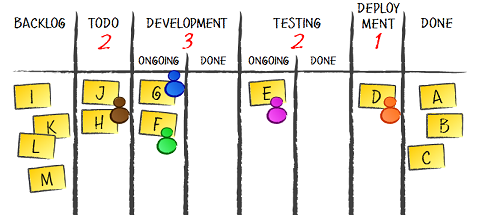
\includegraphics[width=1.0\textwidth]{img/kanban_board.png}
    \captionsource{Image showing the basics of a kanban board. The cards move from left to right. The number under each category represent the \gls{wip} limit. }{Pawel Brodzinski, \url{http://brodzinski.com/}}
    \label{fig:kanban_board}
\end{figure}



\subsection{Visualize}
This practice is about visualizing workflow. To have transparency between developers, managers and anyone else connected to a project. The standard way of doing this is using a so called kanban board with cards, see Figure \ref{fig:kanban_board}. This board can either be a physical board with sticky notes, or a virtual board. This board is a visual control system for all the tasks within a project \cite{key16}. The board allows for self-organizing by just pulling a new available card after finishing a task instead of waiting for a superior to supply the tasks.

The cards are not only meant to simply hold programming tasks. They are meant to represent some customer value. Therefor the design of the cards is important in order for the developers to make easier decisions on what to work on next \cite{key16}. There are no exact rules on what information the cards should hold but a title, description, estimated size and some estimated value number is a good start.

\subsection{Limit Work-in-Progress}
Limiting \gls{wip} is about having a limit at each step in the product chain, shown in Figure \ref{fig:kanban_board}, that corresponds to the amount of tasks allowed in that step. A simple \gls{wip} limit is having it equal to the amount of available working people at each step. When deciding the \gls{wip} limit, all members from from the stake holders to the developers should take part and form an agreement�\cite{key16}. 

The \gls{wip} limit is important for several reasons. It shows when a pull from one step can be made to the next, it ensures focus on one or a few tasks at a time, it keeps the workload balanced and avoids stock piling of items at some middle step in the product chain. The most important benefit is that it gives the development team a limit to rely on and fall back to when put under to much stress, especially if everyone participated and formed a consensus when choosing the limit for the \gls{wip}. 

\subsection{Manage Flow}
In Kanban the workflow or task flow is central so it makes sense having a practice focus on how to manage and improve it. In order to improve the workflow one must first be able to measure it somehow. Otherwise when changes are made, how do we know that it was an improvement? Some things are easier to measure and improve such as items stock piling at a certain step. An easy fix would be to add more manpower to that particular step. Some software such as \emph{Kanbanery} offer automatic tools for measuring that can give useful information about how changes affect the workflow \cite{key18}. Something important to stress out is that the more precise the estimated complexities and values for the cards/tasks the easier it gets to analyze the workflow.

\subsection{Make Process Policies Explicit}
In the practice \emph{Visualize} it was mentioned the importance of having a clear design on the cards of the kanban board. This practice is about just that. Without clear rules and a common understanding of how the card system works the discussions becomes subjective and emotional instead of factual \cite{key19}. Having the process policies explicit makes them easier to understand and therefor easier to use. They help choices regarding the process become more rational and empirical and the team have an easier time reaching consensus simply because everyone is working from the same policy configuration \cite{key19}.


\subsection{Improve Collaboratively}
\epigraph{If you are not continually improving, but you are doing all of the other parts of the Kanban method, you are missing the point. It's a little like the concept of ?doing? agile but not being agile.
. \cite{key19}}{\textsc{Matthew Powell}}

This practice is more social and less practically oriented then the other. When reading about Kanban you sometimes stumble upon the word \emph{Kaizen} meaning continuous improvement. \emph{Kaizen culture} is also often mentioned that talks about empowering the workforce and encourage them to "do the right thing". Kaizen culture promotes high levels of collaborations and freedom to self-organize work \cite{key16}. It is about putting the company and business first and this requires lots of trust which Simon Sinek talk about in his TED Talk about leadership \cite{key7}.

Kanban promotes using a scientific approach when trying to introduce new changes. That means to evaluate a situation, suggest suitable change, predict the outcome, observe the results and compare with the prediction and previous results. If the team or business have a kaizan culture together with using the scientific approach then that can lead to spontaneously and regular local improvements to the process \cite{key16}.


\mypart{Method}{The method is divided in two main parts. The first section describes the theoretical evaluation of agile methodologies. The second part describes the project that has been developed using a few selected agile strategies.}

\chapter{Theoretical Evaluation of Methodologies}
\label{sec:method_teori}

\subsection{Agile Methodology Point System} 

\section{Practical Evaluation of Agile Project}

\subsection{Project Description}
The actual project, to be developed using agile strategies, is a private initiative from Per-Arne Forsberg who has 25 years of successful international experience and knowledge in managing technically skilled units, products and projects around the world at Ericsson. Having been involved and engaged in change management, using the latest Lean and Agile methodology.
The project is developing a dynamic, scalable and robust interactive tutoring framework prototype for pre-academic students. Assisting students today according to the ?old school? is social but also ineffective since it is usually one to one communication or one to a few in a geographical location (you have to meet at pre-determined location at pre-determined times, like classrooms). The long term goal is to assist in communication between students and teachers (tutors willing to help out with their knowledge from their preferred location) in Sweden and in turn combat the negative (knowledge) grade curve that can be seen around the country (according to international studies, PISA). In short the idea is to create a interactive website that can be used for many to many type of communication between students and teachers. An exact specification of the project does not exist in order to encourage the agile development process.

\subsection{Chosen Methodology and/or Strategy}

\mypart{Results}{The results have a similar layout as the method. The first chapter shows the results of the theoretical evaluation. The second part goes through the results of the practical project. }


\chapter{Theoretical}

\section{Point System}

\section{Practical}

\subsection{Project}

\subsection{Developer \& Product Owner Experience}


\mypart{Discussion}{The following chapters will be discussions and final toughs regarding the results, future work, report critique and more.}

\chapter{Discussion}

\chapter{Conclusions}

\chapter{Report Critique}
There are several reasons to be critical for the type of research conducted in this report. Some have already been mentioned briefly here and there throughout the report. First of all agile development by itself is quite vague in its definitions and the work regarding agile development and its methodologies are mostly based on expert experience. It is the results of industry experts that have seen problems, come up with ideas to fix them, had companies or themselves try them out finally evaluate  the outcome. The problem is that there are so many parameters and influences when evaluating software development methodologies that it is really hard to make sense of the result. Too be clear, the data is very noisy. For instance, you can not make a software using one methodology and then have the development team create the software again using another approach. The results of the new approach will most certainly be influenced by their first attempt. What is really needed is several development teams consisting of developers with somewhat equal experience and background. However, depending on parameters such as if the software type is a website, game or security system the results might vary. Thus most work regarding agile development and its methodologies, including this report, falls into the category of social science or soft science which is important to have in mind. All of this also means that investigating work regarding agile development, such as this report, would benefit in having a more experienced author but this is usually hard to come around when we talk about a university thesis for obvious reasons.

Each agile development methodology has vast amount of information, interpretations and alternative versions going for them. To make a full theoretical analyzes and comparison is out of scope for this report. The first and easy limitation was to not include every possible agile methodology in order to have room for more depth into the chosen methodologies as well as to keep the complexity down and give the readers some focus. However, even with this limitation it would not be viable going through every aspect of each methodology since each methodology would deserve their own full report. So the practices of each methodology was chosen as a solid and common ground to be analyzed. What this means is that a lot of what defines the methodologies have potentially been "cut off" and therefore given an unfair assessment to some degree. This is also brought up in \fullref{sec:future_work}.

 

\chapter{Developers Thoughts}

\section{Future Work} 
\label{sec:future_work}


\printglossary[type=main]
\nopagebreak[4]
\printglossary[type=\acronymtype]


\appendix
\addappheadtotoc
\chapter{RDF}\label{appA}

\begin{figure}[ht]
\begin{center}
And here is a figure
\caption{\small{Several statements describing the same resource.}}\label{RDF_4}
\end{center}
\end{figure}

that we refer to here: \ref{RDF_4}

\begin{thebibliography}{56}

\bibitem{key1}
Martin C. Robert, Martin Micah,
\emph{Agile Principles, Patterns, and Practices in C\#}.
Prentice Hall, Massachusetts,
2nd edition,
2006.

\bibitem{key2}
\url{http://www.agilealliance.org}

\bibitem{key3}
\url{https://www.youtube.com/watch?v=t9YLtDJZtPY&t=175}

\bibitem{key4}
\url{http://www.literateprogramming.com/knuthweb.pdf}

\bibitem{key5}
\url{http://users.dcc.uchile.cl/~nbaloian/cc1001-03/ejercicios/crystalclearV5d.pdf}

\bibitem{key6}
[KW] Karl Weick, The Social Psychology of Organizing, McGraw-Hill Humanities/Social Sciences/Languages; 2nd edition, 1979.

\bibitem{key7}
\url{http://www.ted.com/talks/simon_sinek_why_good_leaders_make_you_feel_safe}

\bibitem{key8}
Keil, M. and Carmel, E. (1995) Customer Developer Links in Software Development, Communications of the ACM, Vol 38, Num 5, May. pp33-44

\bibitem{key9}
[Cockburn2001] Alistair Cockburn and Laurie Williams, "The Costs and Benefits of Pair
Programming," XP2000 Conference in Sardinia, reproduced in Giancarlo Succi and Michele Marchesi,
Extreme Programming Examined, Addison-Wesley, 2001.

\bibitem{key10}
[Nosek98] J. T. Nosek, "The Case for Collaborative Programming," Communications of the ACM,
1998, pp. 105108.

\bibitem{key11}
[Williams2000] Laurie Williams, Robert R. Kessler, Ward Cunningham, Ron Jeffries, "Strengthening
the Case for Pair Programming," IEEE Software, JulyAug. 2000.

\bibitem{key12}
\url{https://people.kth.se/~tomase/#/presentations/computer_science}

\bibitem{key13}
\url{http://repo.hackerzvoice.net/depot_madchat/coding/xp/xpexplained.pdf}

\bibitem{key14}
\url{http://ptgmedia.pearsoncmg.com/images/9780321278654/samplepages/9780321278654.pdf}

\bibitem{key15}
\url{http://www.scrumguides.org/scrum-guide.html}

\bibitem{key16}
\url{http://www.scrumsense.com/wp-content/uploads/2010/02/KanbanManuscript-dja-rev1_07_2.pdf}

\bibitem{key17}
\url{http://en.wikipedia.org/wiki/Kanban}

\bibitem{key18}
\url{https://kanbanery.com/ebook/GettingStartedWithKanban.pdf}

\bibitem{key19}
\url{http://www.everydaykanban.com/what-is-kanban/}

\bibitem{key20}
\url{https://www.google.se/books?hl=sv&lr=&id=6O5tAgAAQBAJ&oi=fnd&pg=PR3&dq=scrum&ots=1FXoZqQl5Z&sig=oAaGuCqYT8GOPb3L4u6kqIoWYH8&redir_esc=y#v=onepage&q=jeff%20sutherland&f=false} %About combining xp with scrum

\bibitem{key21}
\url{https://www.google.se/url?sa=t&rct=j&q=&esrc=s&source=web&cd=1&ved=0CCUQFjAA&url=http%3A%2F%2Fxa.yimg.com%2Fkq%2Fgroups%2F19611210%2F134287803%2Fname%2FAgile&ei=MXsRVeqRMeHXyQOJtoCoDA&usg=AFQjCNEBuHLF_m23E8qOTsBJvOtetCxukw&sig2=J3vpAfBnP0Mhms92bnycIA&bvm=bv.89184060,d.bGQ&cad=rja}

\bibitem{key22}
2. J. Womack, D. Jones, and D. Roos, The Machine
That Changed the World: The Story of
Lean Production, Simon \& Schuster, 2007

\bibitem{key23}
http://ptgmedia.pearsoncmg.com/images/9780321150783/samplepages/0321150783.pdf

\bibitem{key24}
http://martinfowler.com/bliki/AgileVersusLean.html

\end{thebibliography}

\end{document}
